\documentclass{atistandalonetask}
\usepackage{atistandard}
\begin{document}
  \begin{atiTask}[
    title = Füllung eines Tankwagens
  ]
  
  Der Tank eines Tanklastwagens hat die Form eines liegenden elliptischen Zylinders, der sich durch
  \[
  \frac{x^2}{a^2}+\frac{y^2}{b^2}=1,\quad 0\leq z\leq L
  \]
  beschreiben lässt.Geben Sie das Volumen der getankten Flüssigkeit in Abhängigkeit von der Füllhöhe $0\leq h\leq 2b$ an, indem Sie das zugehörige Volumenintegral lösen.
  \begin{figure}[H]
\centering
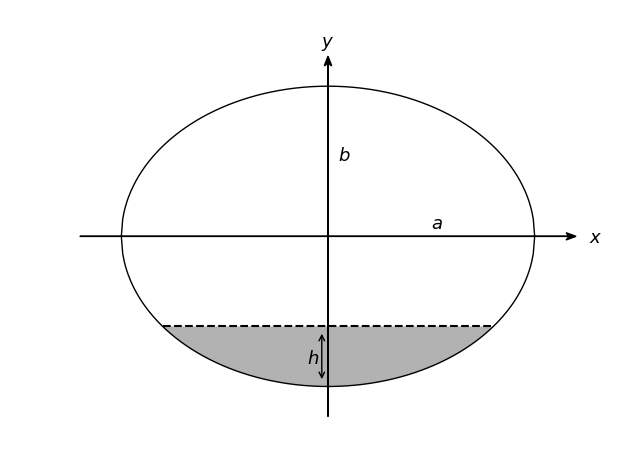
\includegraphics[width=0.7\linewidth]{./picture-doppelintegral_iii}
\caption{Tankwagenquerschnitt}

\end{figure}

  	
  \end{atiTask}
  \begin{atiSolution}
   	Lösung folgt
  	%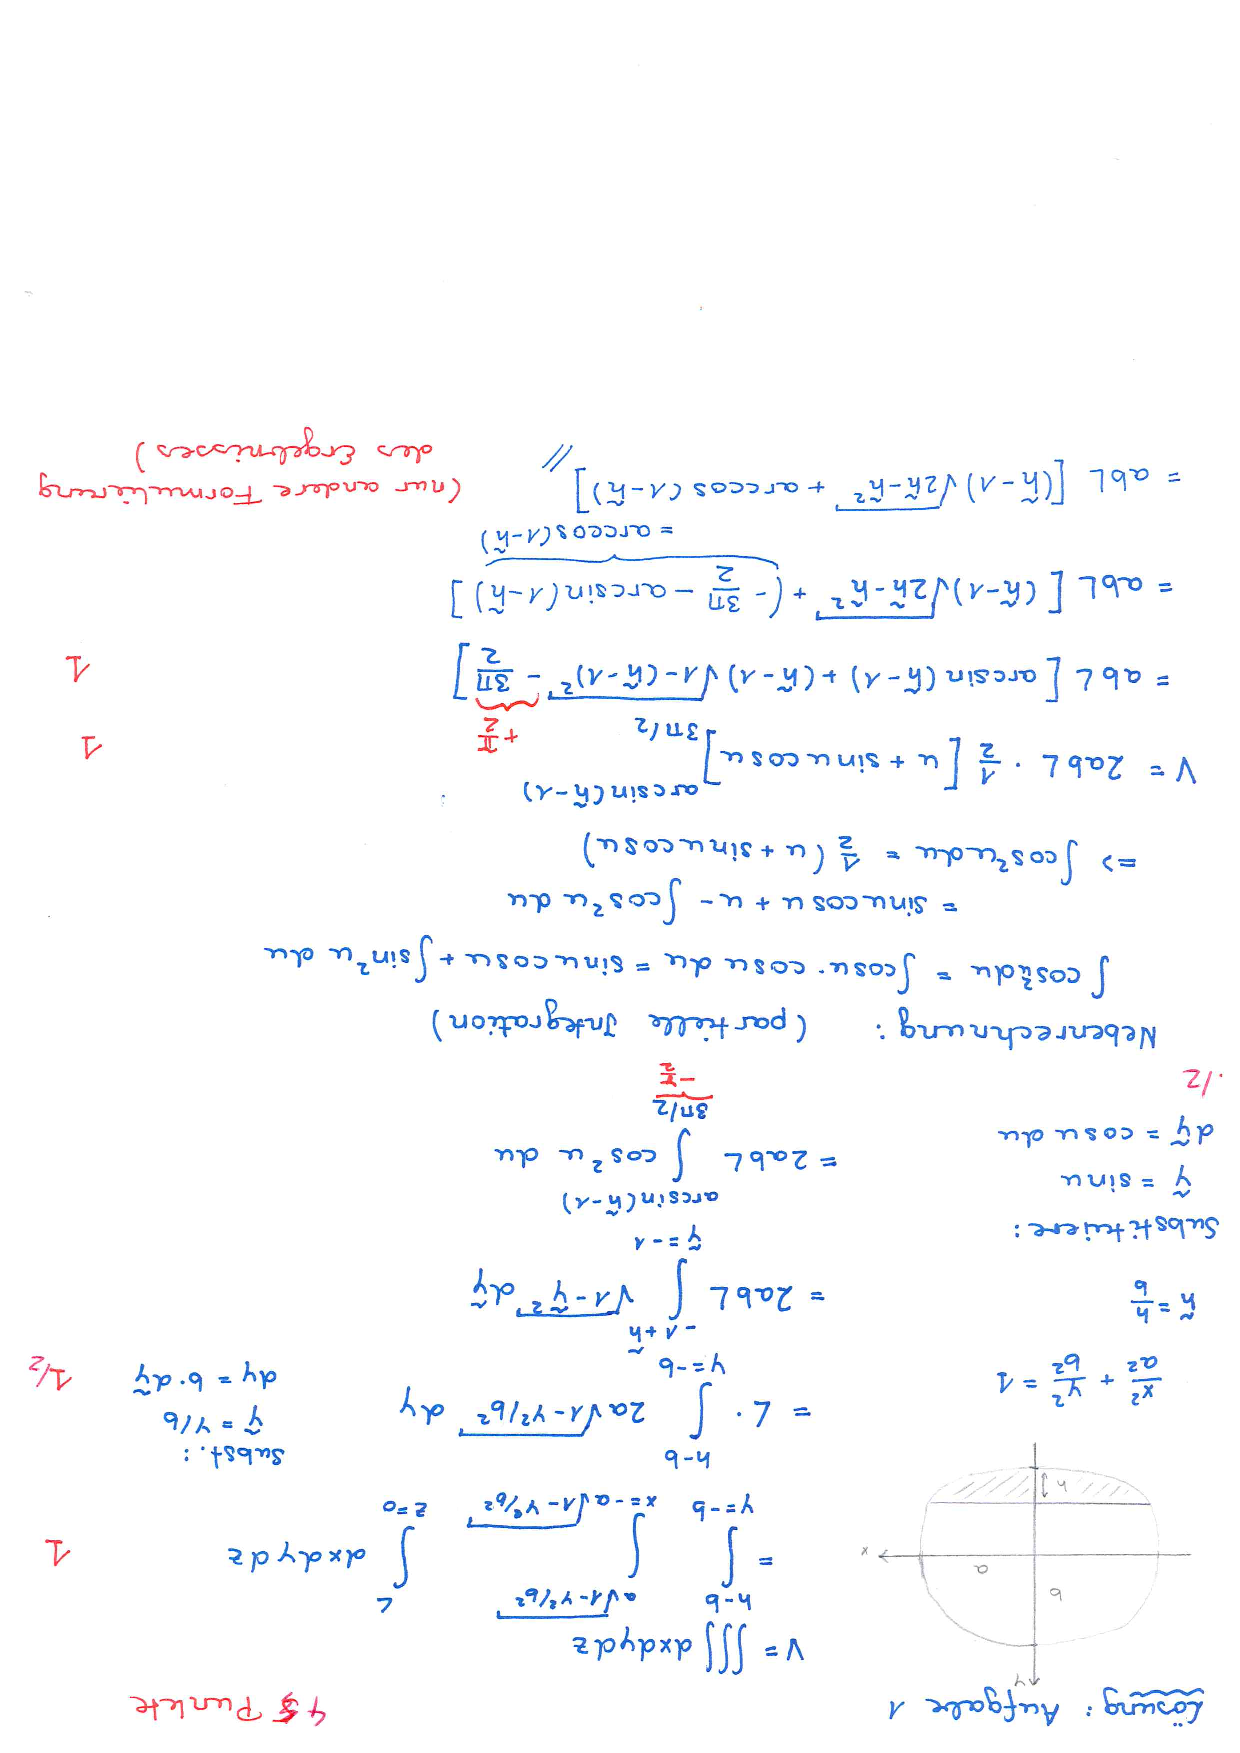
\includepdf[pages=-]{solution-doppelintegral_iii.pdf}
  \end{atiSolution}
\end{document}